\documentclass[10pt]{beamer}

\usetheme[progressbar=frametitle, sectionpage=none]{metropolis}
\usepackage{appendixnumberbeamer}
\usepackage{pgfpages}
\usepackage{booktabs}
\usepackage[dvipsnames]{xcolor}
\usepackage{mathtools}

\usepackage{pgfplots}

\usepgfplotslibrary{dateplot}

\setbeameroption{slides only}
%\setbeameroption{show only notes}
%\setbeameroption{show notes on second screen=right}
\usepackage{xspace}
\newcommand{\themename}{\textbf{\textsc{metropolis}}\xspace}

\title{Labor Markets and Technological Change: Evidence from Electronic Health Records}

\subtitle{Hanna Glenn\\ \small Emory University}
 \date{\today}

\setbeamertemplate{caption}{\raggedright\insertcaption\par}
\setbeamertemplate{itemize item}{\scalebox{.6}{$\blacktriangleright$ }}     
\setbeamertemplate{itemize subitem}{\scalebox{.8}{$\centerdot$ }} 

\begin{document}

\maketitle

\setbeamercolor{background canvas}{bg=white}




\section[Motivation]{Motivation}

\begin{frame}{Big Picture}
How does technology impact employment?

    \begin{itemize}
        \item Displacement?
        \vspace{2mm}
        \item Productivity?
    \end{itemize}
    \vspace{3mm}
    
Investigated in different ways

    \begin{itemize}
        \item Computerization on white collar jobs
        \vspace{2mm}
        \item Machines on factory workers
    \end{itemize}
    
    \vspace{3mm}
    
    \pause
    
    \begin{alertblock}{$\rightarrow$ This paper considers this question in the context of healthcare and physician labor markets}\end{alertblock}
\end{frame}



\begin{frame}[fragile]{What is an Electronic Health Record (EHR)?}
``An electronic health record is the systematized collection of patient and population electronically stored health information in a digital format"

\vspace{5mm}
\centering
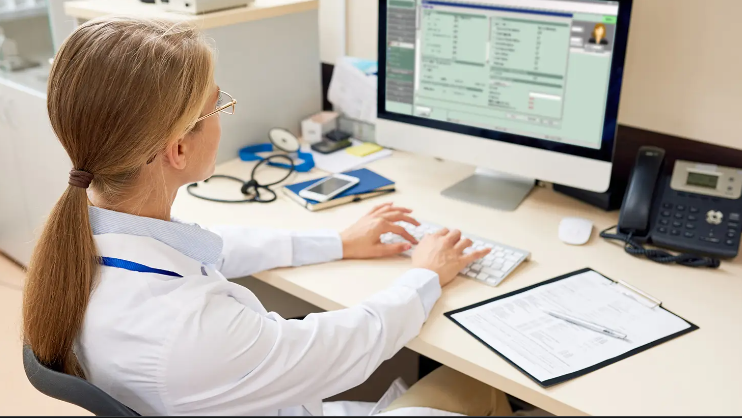
\includegraphics[scale=.35]{Objects/EHR_picture.PNG}
\end{frame}



\begin{frame}[fragile]{HIT: Great (Expected) Potential in Healthcare}
\begin{alertblock}{Cost Saving}
\begin{itemize}
    \item Possible cost reduction of hundreds of billions of dollars \\ \scriptsize (Hillestad et al 2005)
\end{itemize}
\end{alertblock}

\begin{alertblock}{Quality Improvement}
\begin{itemize}
    \item Improved efficiency, patient safety improvements, physicians have decision support that could prevent unnecessary complications, etc.
\end{itemize}
\end{alertblock}

\vspace{4mm}

Significant policy push for EHR implementation: HITECH Act, 2008 provided financial incentive for hospitals to implement EHRs
\begin{itemize}
    \item \textcolor{blue}{The percentage of hospitals with basic EHR capability rose from 9$\%$ in 2008 to 84$\%$ in 2015.} \scriptsize (Health IT Dashboard)
\end{itemize}
\end{frame}




\begin{frame}{Physician Response to EHRs}
\begin{center}
    
\includegraphics[scale=.3]{graphics/News Clip3.PNG}
    
    \vspace{3mm}
    
    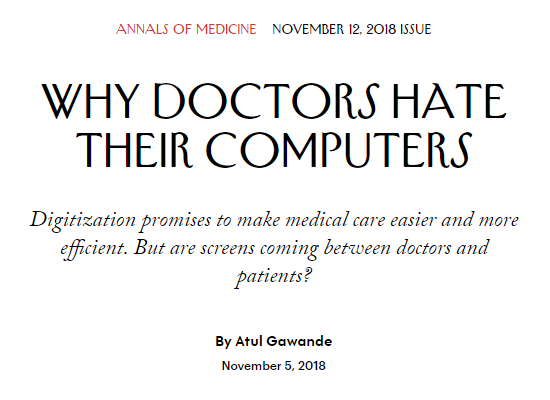
\includegraphics[scale=.3]{graphics/News Clip2.PNG}
\end{center}
\end{frame}




\begin{frame}{This Paper}
$\rightarrow$ Did EHR implementation in hospitals affect physician labor market decisions?

\vspace{5mm}
\centering
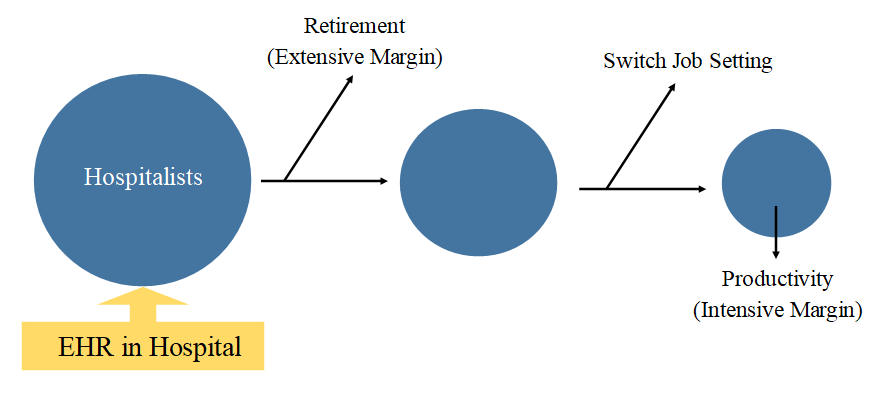
\includegraphics[scale=.45]{Objects/EHR_FlowChart_General.PNG}
\end{frame}



\section{Analysis and Data}




\begin{frame}{Difference in Difference Analysis}
Treatment: Exposure to EHR

\vspace{3mm}

Since I have differential timing of exposure, I use Callaway and Sant'Anna (2021) average group time treatment effects

$$ATT(g,t)=\mathbbm{E}[Y_t(g)-Y_t(0)|G_g=1]$$

\vspace{3mm}

\begin{itemize}
\item Not-yet-treated units as control group
    \item Aggregate these over groups to get a familiar event study plot
\end{itemize}
\end{frame}



\begin{frame}{Data}
Panel of hospitalists from 2009-2017 with information on whether the hospital uses an EHR and various labor market outcomes

\vspace{4mm}
\pause
\begin{itemize}
    \item EHR information ends in 2015, so I limit to only those who were exposed by 2015
\end{itemize}
\end{frame}

\begin{frame}{Data}
    \centering
    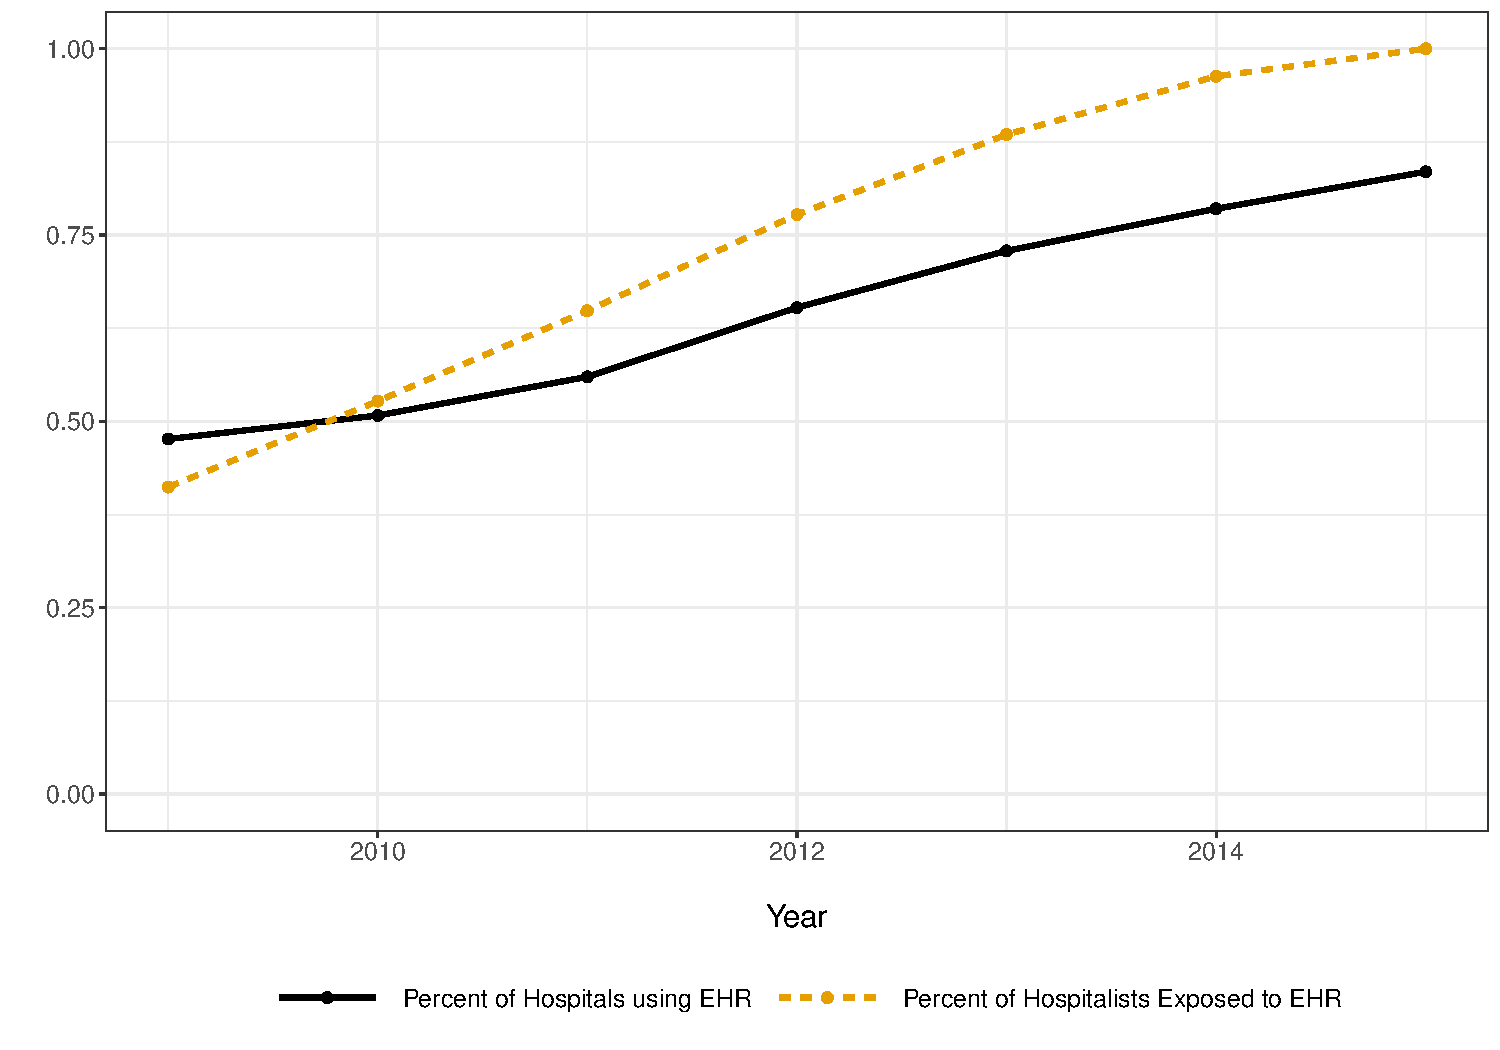
\includegraphics[scale=.4]{Objects/sum_stats_year.pdf}
\end{frame}


\begin{frame}{Assumptions}
\begin{enumerate}
    \item No reversal of treatment
    \vspace{3mm}
    \item No anticipation of treatment (can be relaxed)
    \vspace{3mm}
    \item Parallel trends
\end{enumerate}
\end{frame}


\section{Retirement}



\begin{frame}{Retirement}
    \centering
    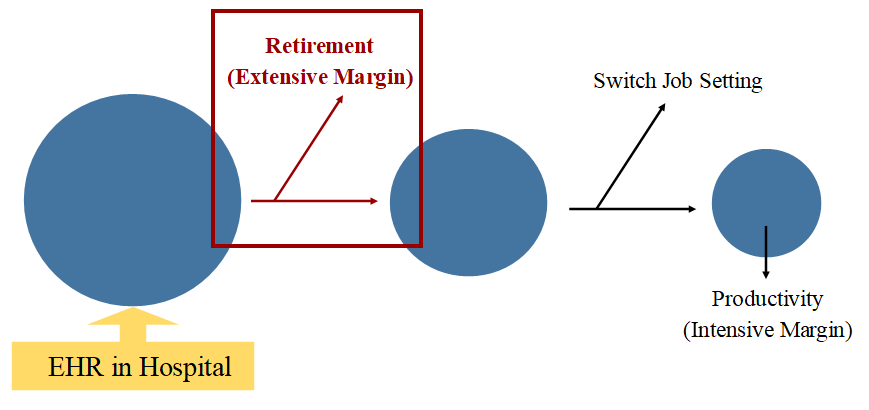
\includegraphics[scale=.5]{Objects/EHR_FlowChart_Retire.PNG}
\end{frame}

\begin{frame}{Retirement Variable}
Indicator variable equal to 1 if the physician drops out of the data 
\vspace{3mm}
\begin{itemize}
    \item No longer seeing patients
\end{itemize}
\end{frame}



\begin{frame}{Physician Incentives}
Decision to retire is different than we usually think of
\vspace{3mm}
    \begin{itemize}
        \item Retirement is thought of as a function of pensions, and sometimes depends on shocks such as health or job loss
        \tiny (Hall and Johnson 1980, ILRR), (Gordon and Blinder 1980, J Public Econ), (Hamermesh 1985, JOLE), $\cdot$
        
        \vspace{3mm}
    
        \normalsize \item On average, physicians plan to retire at age 60 but don't actually retire until age 69 \tiny(Collier 2017)
    \end{itemize}
    
\vspace{3mm}
\pause

\normalsize Unique set of incentives for which a shock to the work setting \textit{may} lead to retirement more-so than other occupations, for which studies yield mixed results  \tiny (Schleife 2006, Labour; Cavapozzi et al 2013, AE; Roger et al 2006, EJ; Friedburg 2003, ILRR)

\vspace{3mm}
\pause

\normalsize Related studies find that well educated workers exited at higher rates due to computerization \tiny (Willis and Hudomiet 2021, Labour), (Dillender & Forsythe 2022, NBER)
\end{frame}



\begin{frame}{Leaving Clinical Setting}
    \begin{itemize}
        \item Retirement is loosely defined
        \vspace{5mm}
        \item Any age physician may decide to leave a clinical setting
    \end{itemize}
\end{frame}

\begin{frame}{Retirement}
\begin{figure}[ht]
    \centering
    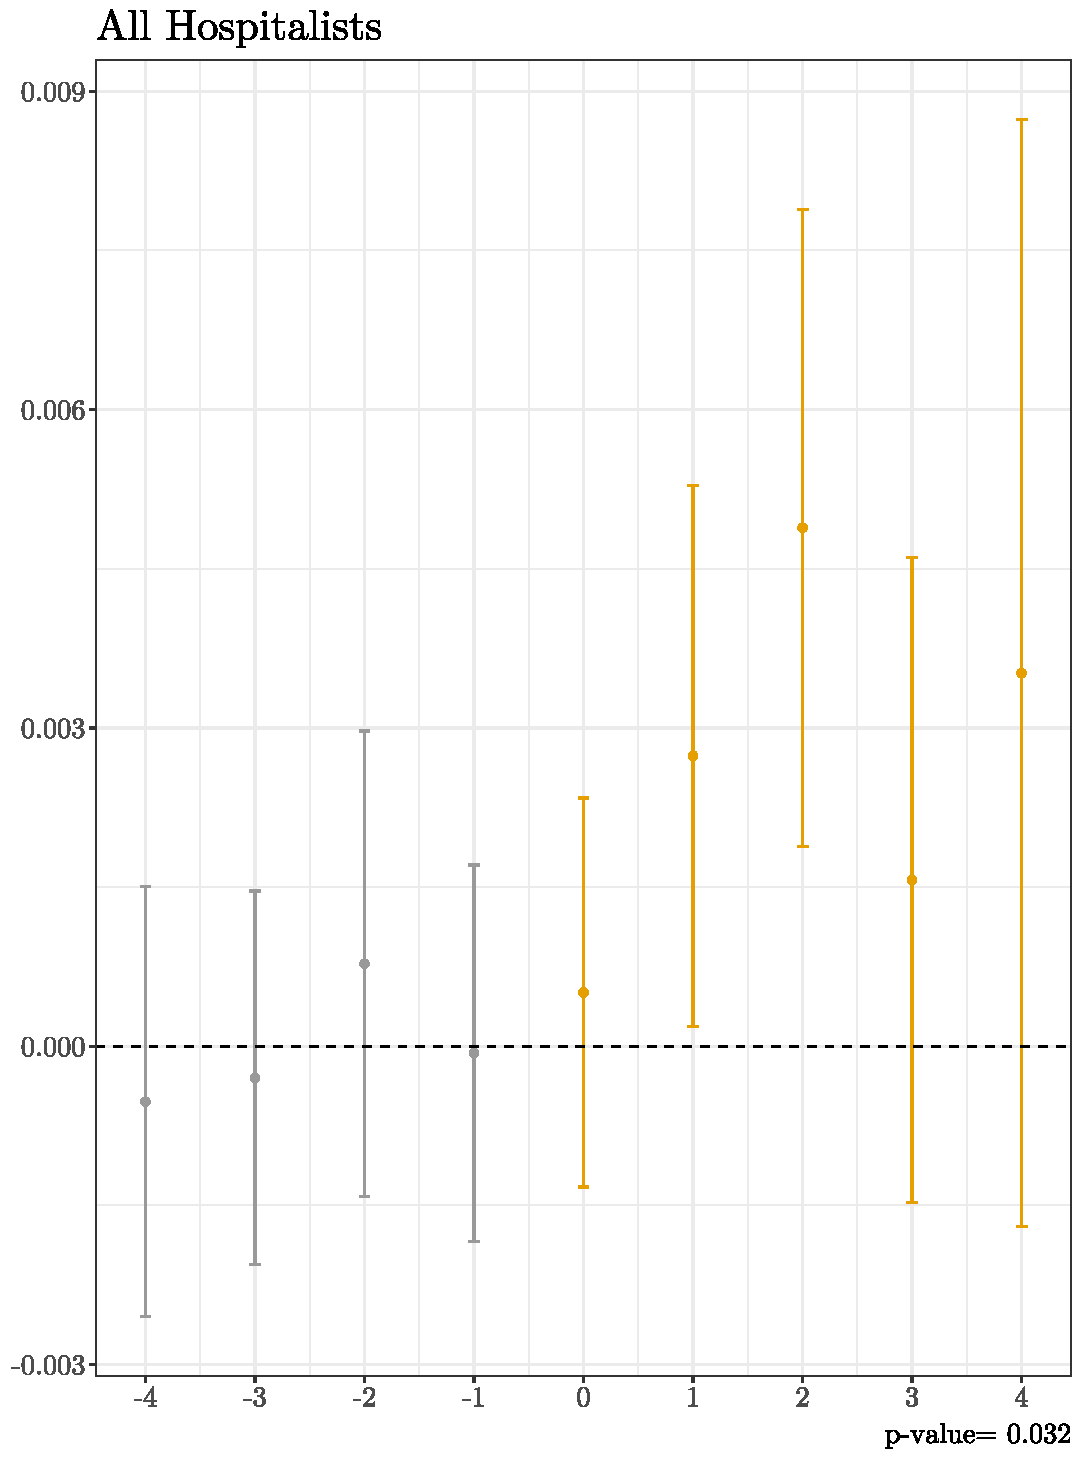
\includegraphics[scale=.35]{Objects/Presentation_retire_all.pdf}
\end{figure}
$\rightarrow$ EHR exposure led to a .003 (.0045) percentage point increase in the likelihood of retirement in the first (second) year after exposure (10\% and 15\% increase relative to the mean)
\end{frame}

\begin{frame}{Retirement: Senior Physicians}
\begin{figure}[ht]
    \centering
    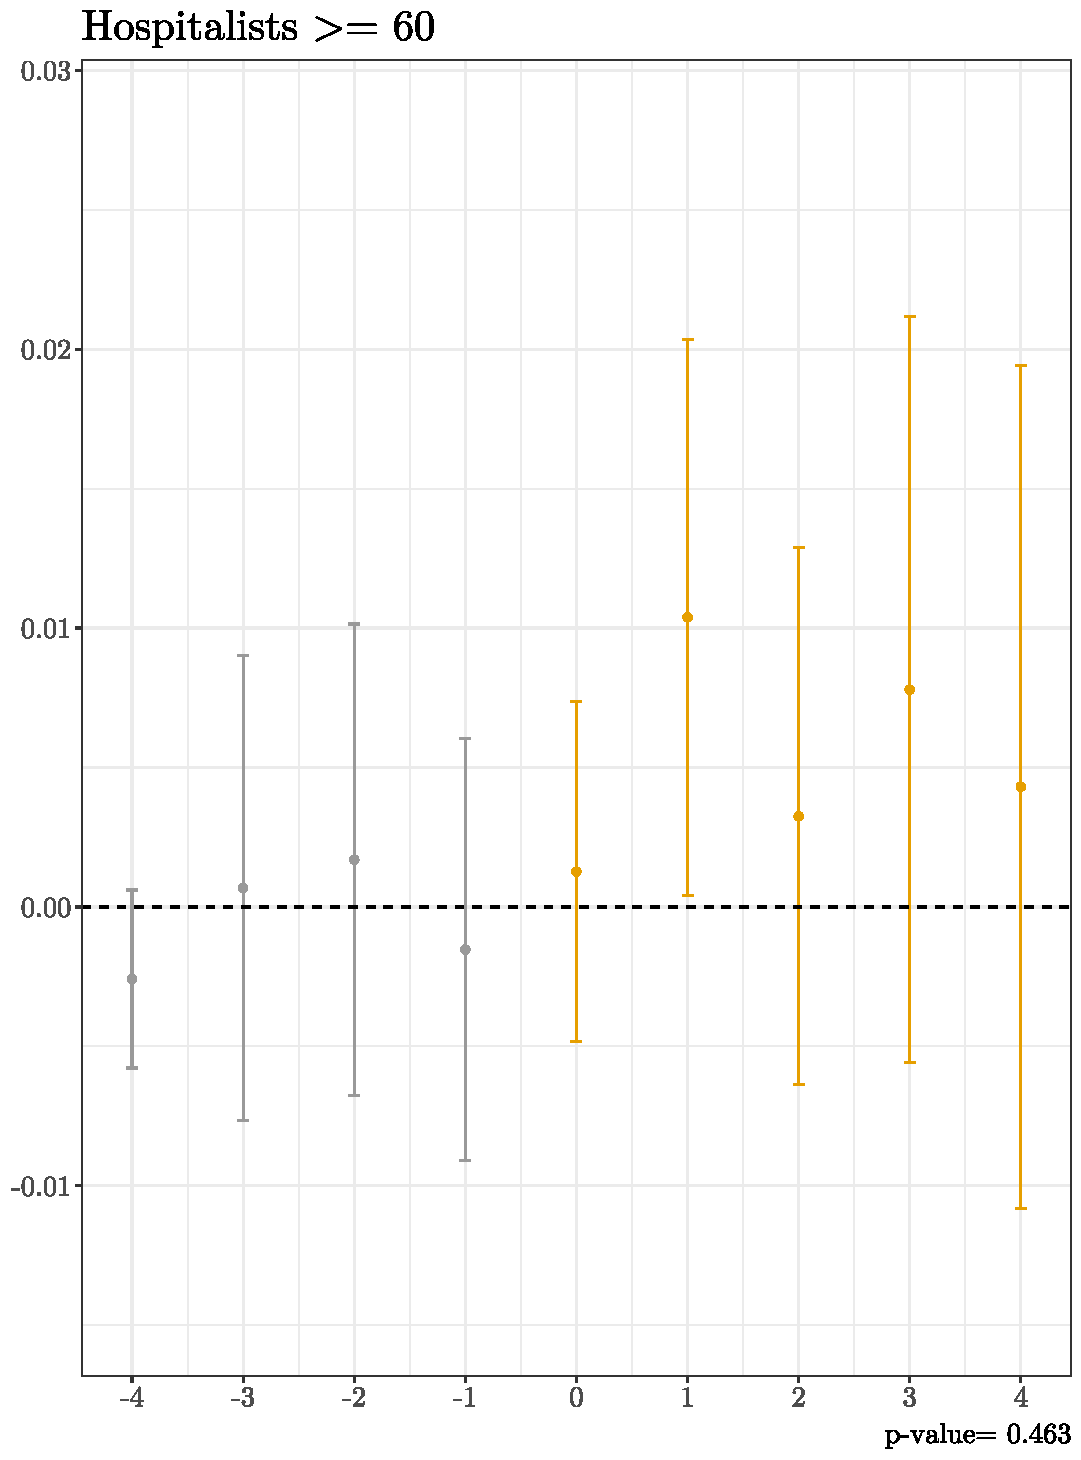
\includegraphics[scale=.35]{Objects/Presentation_retire_old.pdf}
\end{figure}
$\rightarrow$ 25\% increase relative to the mean in the first year, but 0 in the second\\
$\rightarrow$ What does this mean for younger physicians?
\end{frame}





\section{Job Setting}




\begin{frame}{Changing Job Setting}
    \centering
    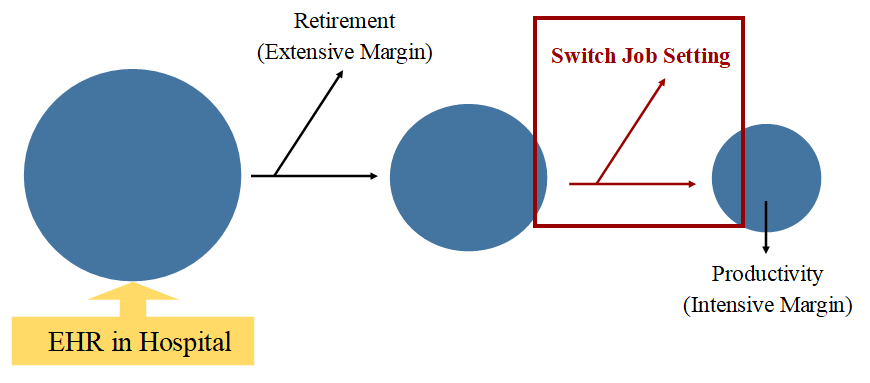
\includegraphics[scale=.5]{Objects/EHR_FlowChart_JobSwitch.PNG}
\end{frame}

\begin{frame}{Job Switching Variables}
    \begin{enumerate}
        \item Fraction of Patients Seen in Office 
        \vspace{3mm}
        \item Indicator for working in office or not
    \end{enumerate}
\end{frame}



\begin{frame}{Physician Incentives}
Most physicians will not be induced to retire because of EHRs
    \begin{itemize}
        \item Another way to avoid (or be exposed to) new technology is to switch location of practice
        \begin{itemize}
            \vspace{3mm}
            \item Literature shows job switching is closely tied to job satisfaction \tiny (Aklerlof, Rose and Yellen 1988, Brookings), (Chadi and Hetschko 2017, JEMS)
        \end{itemize}
        \vspace{6mm}
        \pause
        \item The cost associated with switching depends on the strength of the tie with the hospital
    \end{itemize}
\end{frame}

\begin{frame}{Fraction of Patients Seen in Office}
\begin{figure}[ht]
    \centering
    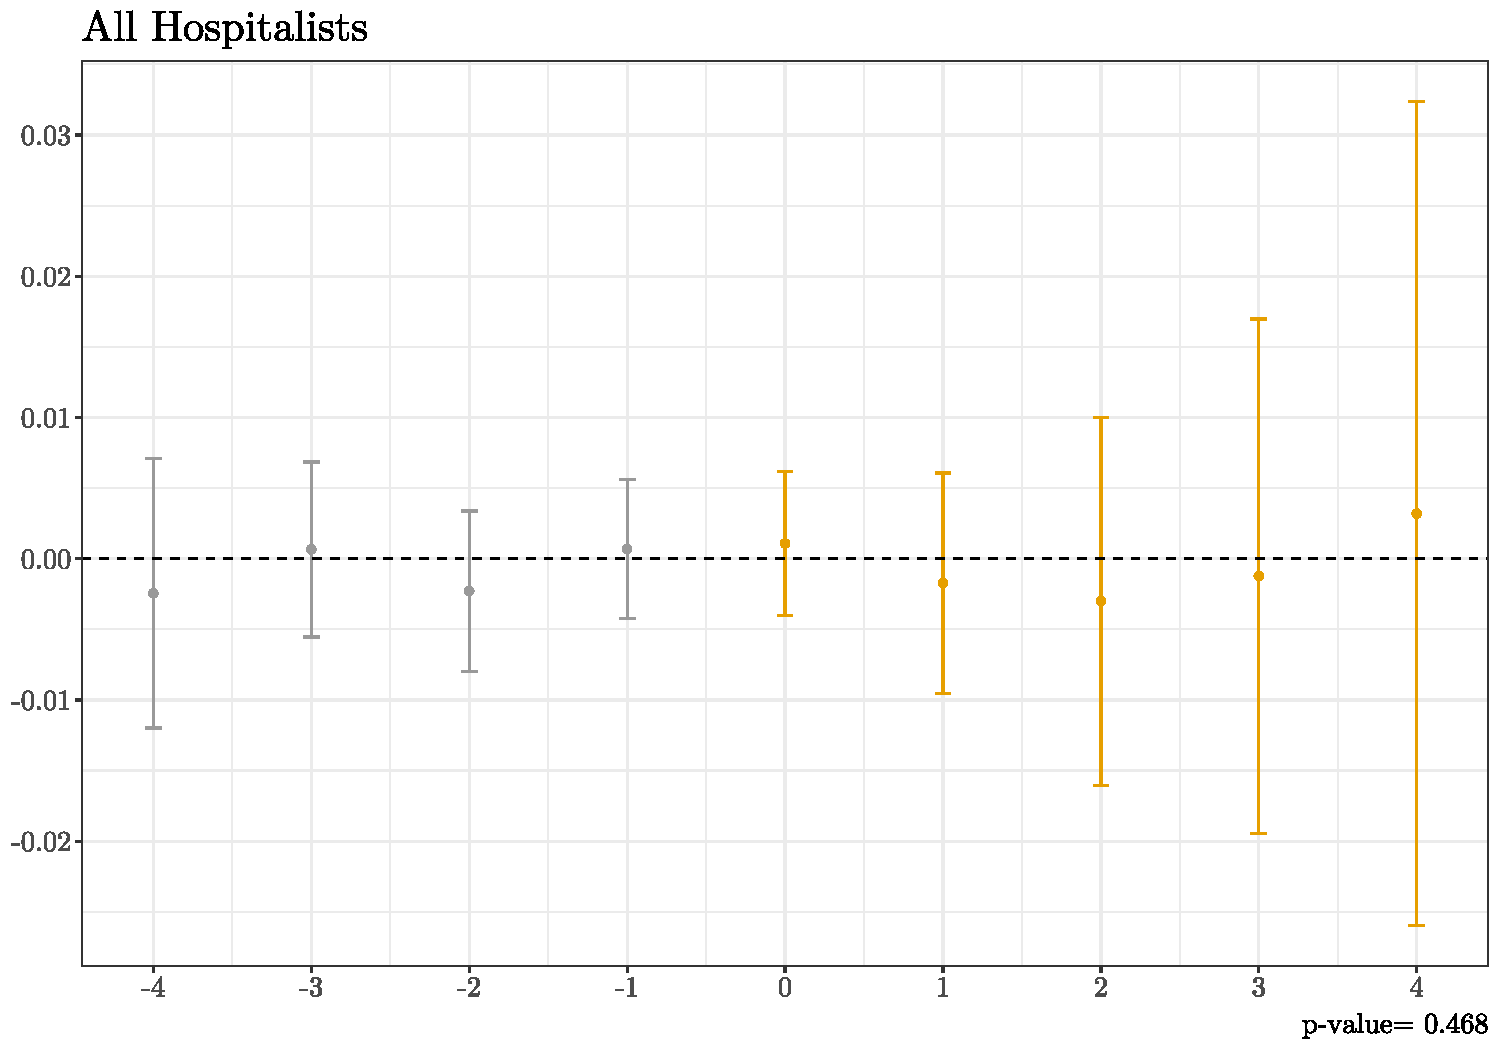
\includegraphics[scale=.35]{Objects/Presentation_fracoffice_all.pdf}
\end{figure}
$\rightarrow$ No effect!
\end{frame}

\begin{frame}{Indicator for working in office}
\begin{figure}[ht]
    \centering
    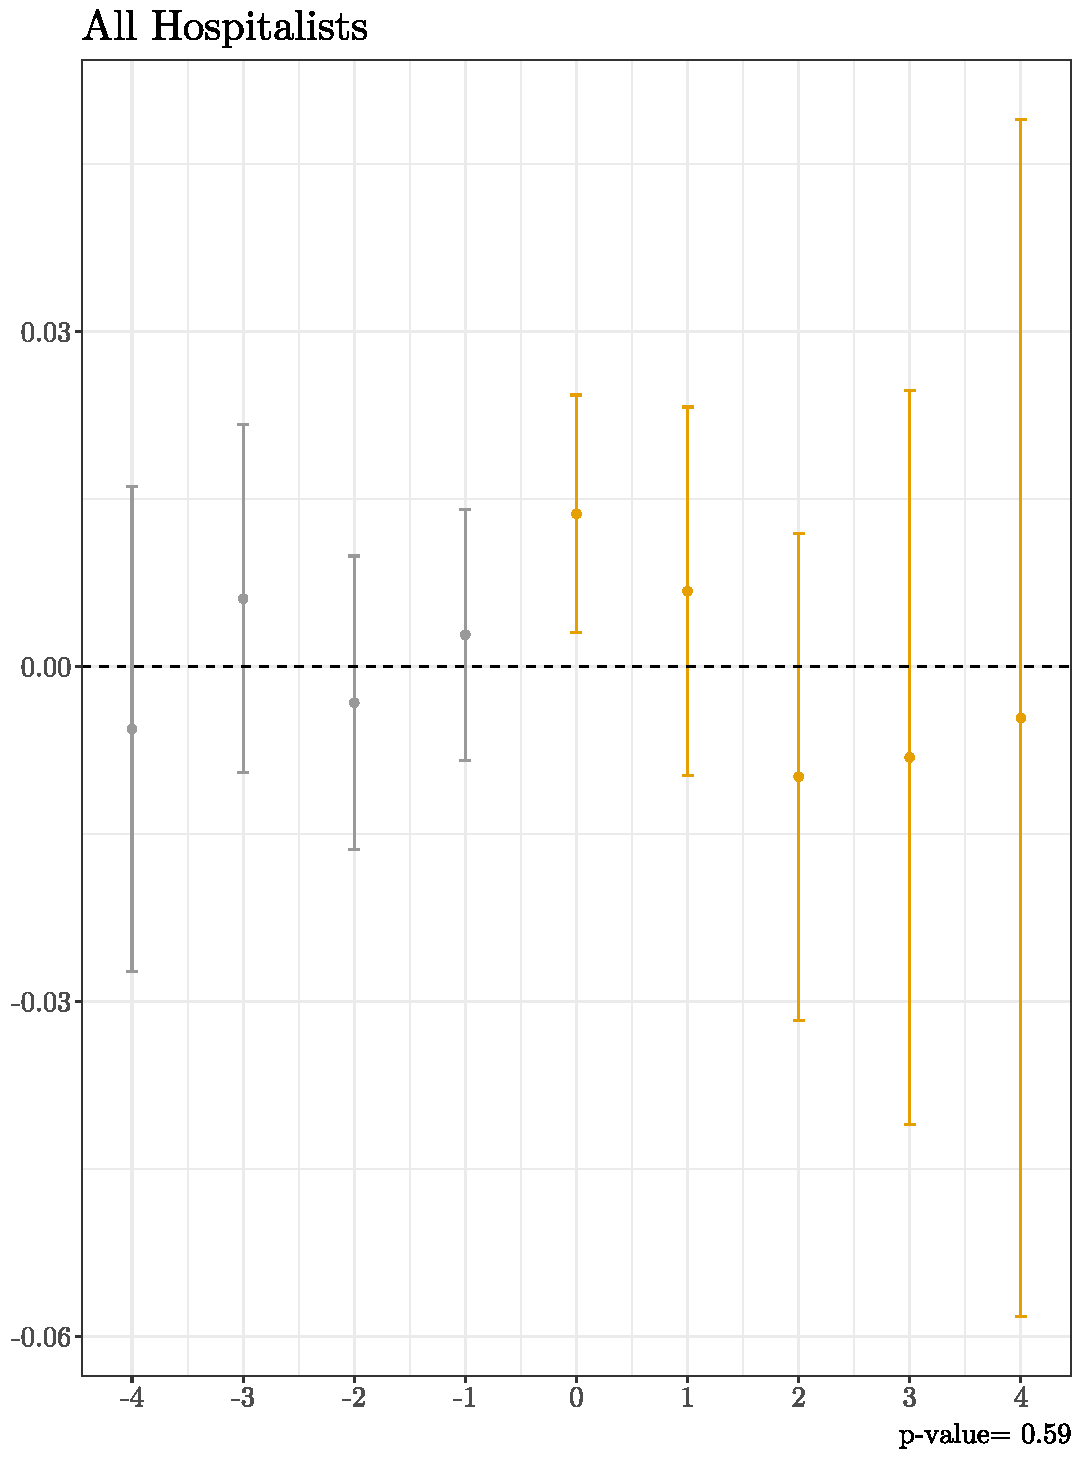
\includegraphics[scale=.35]{Objects/Presentation_office_all.pdf}
\end{figure}
$\rightarrow$ 4.6\% increase relative to the mean\\
$\rightarrow$ Driven by young physicians
\end{frame}





\section{Productivity}





\begin{frame}{Productivity}
    \centering
    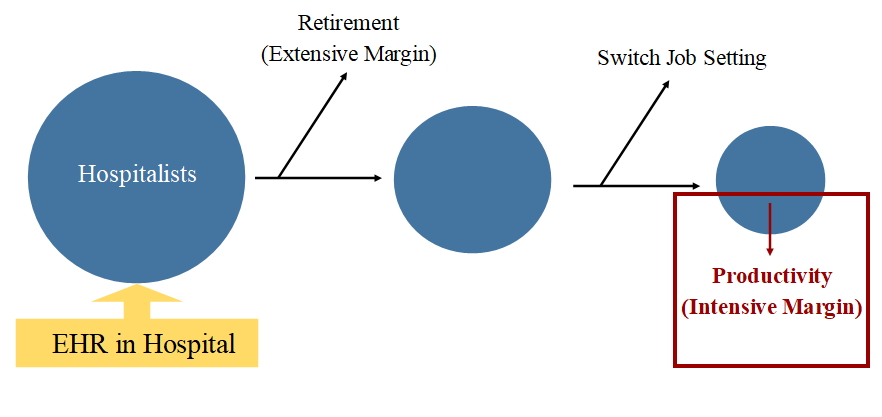
\includegraphics[scale=.45]{Objects/EHR_FlowChart_Productivity.PNG}
\end{frame}

\begin{frame}{Productivity Variables}
    \begin{enumerate}
        \item Patient Count
        \vspace{6mm}
        \item Claims per patient
    \end{enumerate}
\end{frame}

\begin{frame}{Physician Incentives}
Past research on information technology $\rightarrow$ productivity typically indicates increase \tiny (Bartel, Ichniowski and Shaw 2007, QJE)
\vspace{3mm}
\begin{itemize}
    \normalsize \item Sometimes depends on managerial style \tiny(Garicano and Heaton 2010, JLE)
\end{itemize}

\vspace{6mm}

\normalsize We can see how productivity is affected for physicians who don't change behavior as a result of EHRs
\vspace{3mm}
    \begin{itemize}
        \item Expected effect is ambiguous
        \vspace{3mm}
        \item Claim Count per patient is a matter of physician incentives
    \end{itemize}
\end{frame}

\begin{frame}{Patient Count}
\begin{figure}[ht]
    \centering
    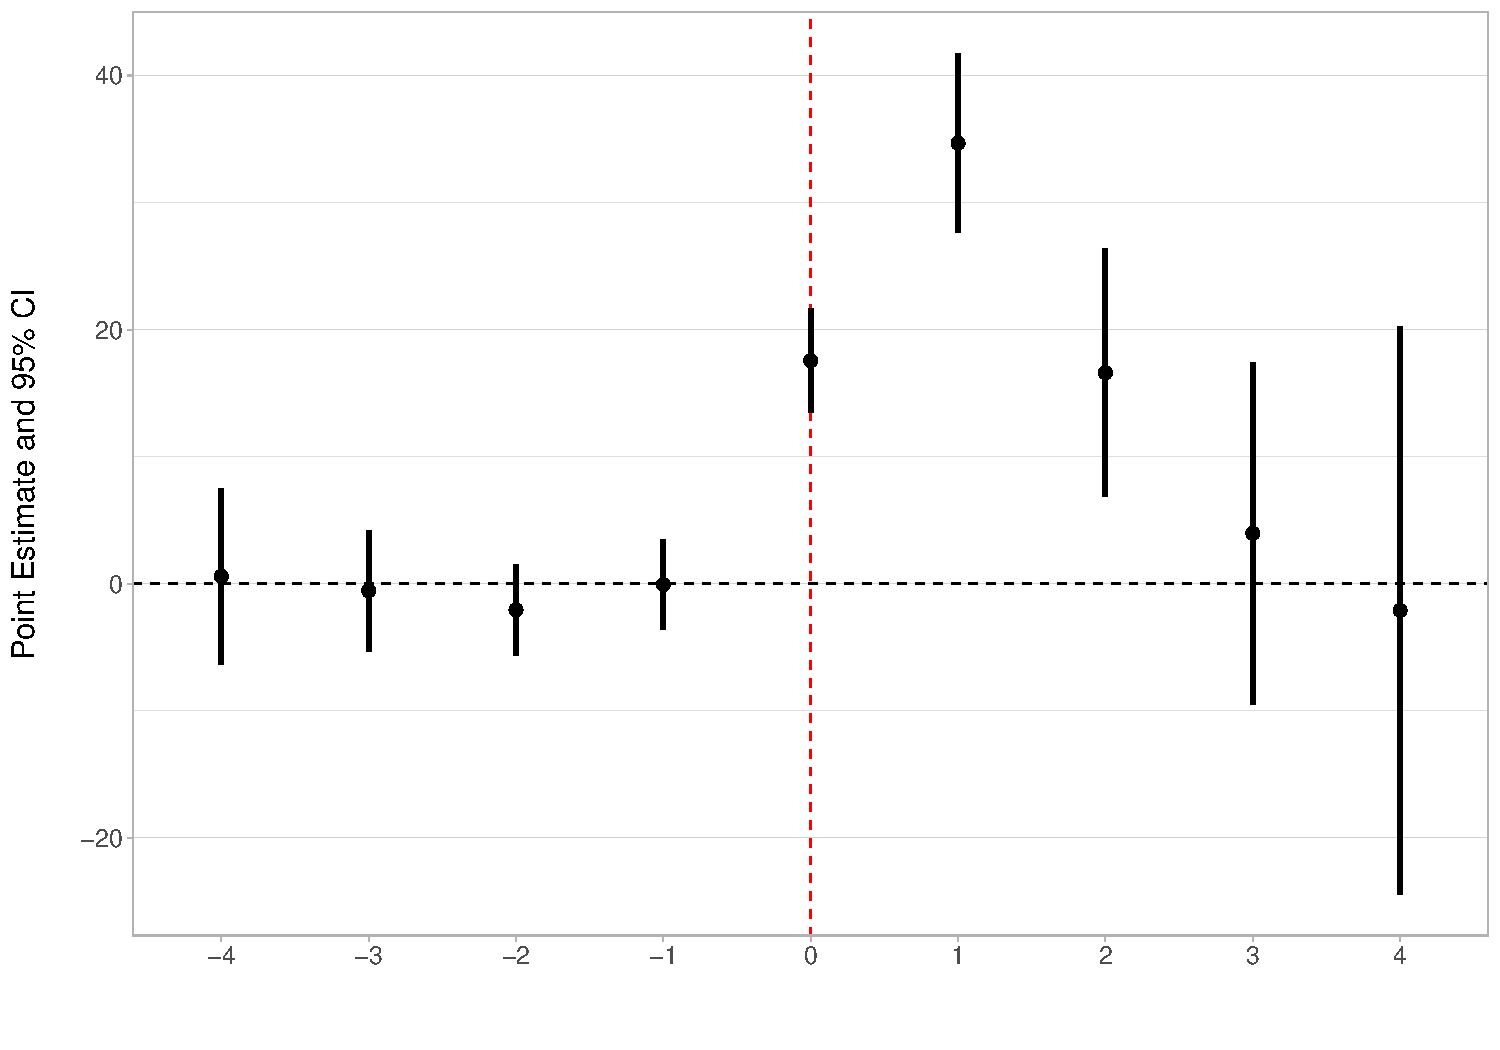
\includegraphics[scale=.35]{Objects/Presentation_patients_all.pdf}
\end{figure}
$\rightarrow$ 5-10\% increase relative to the mean\\
$\rightarrow$ Driven by demand? 
\end{frame}

\begin{frame}{Patient Count Broken Down by Group}
\centering
    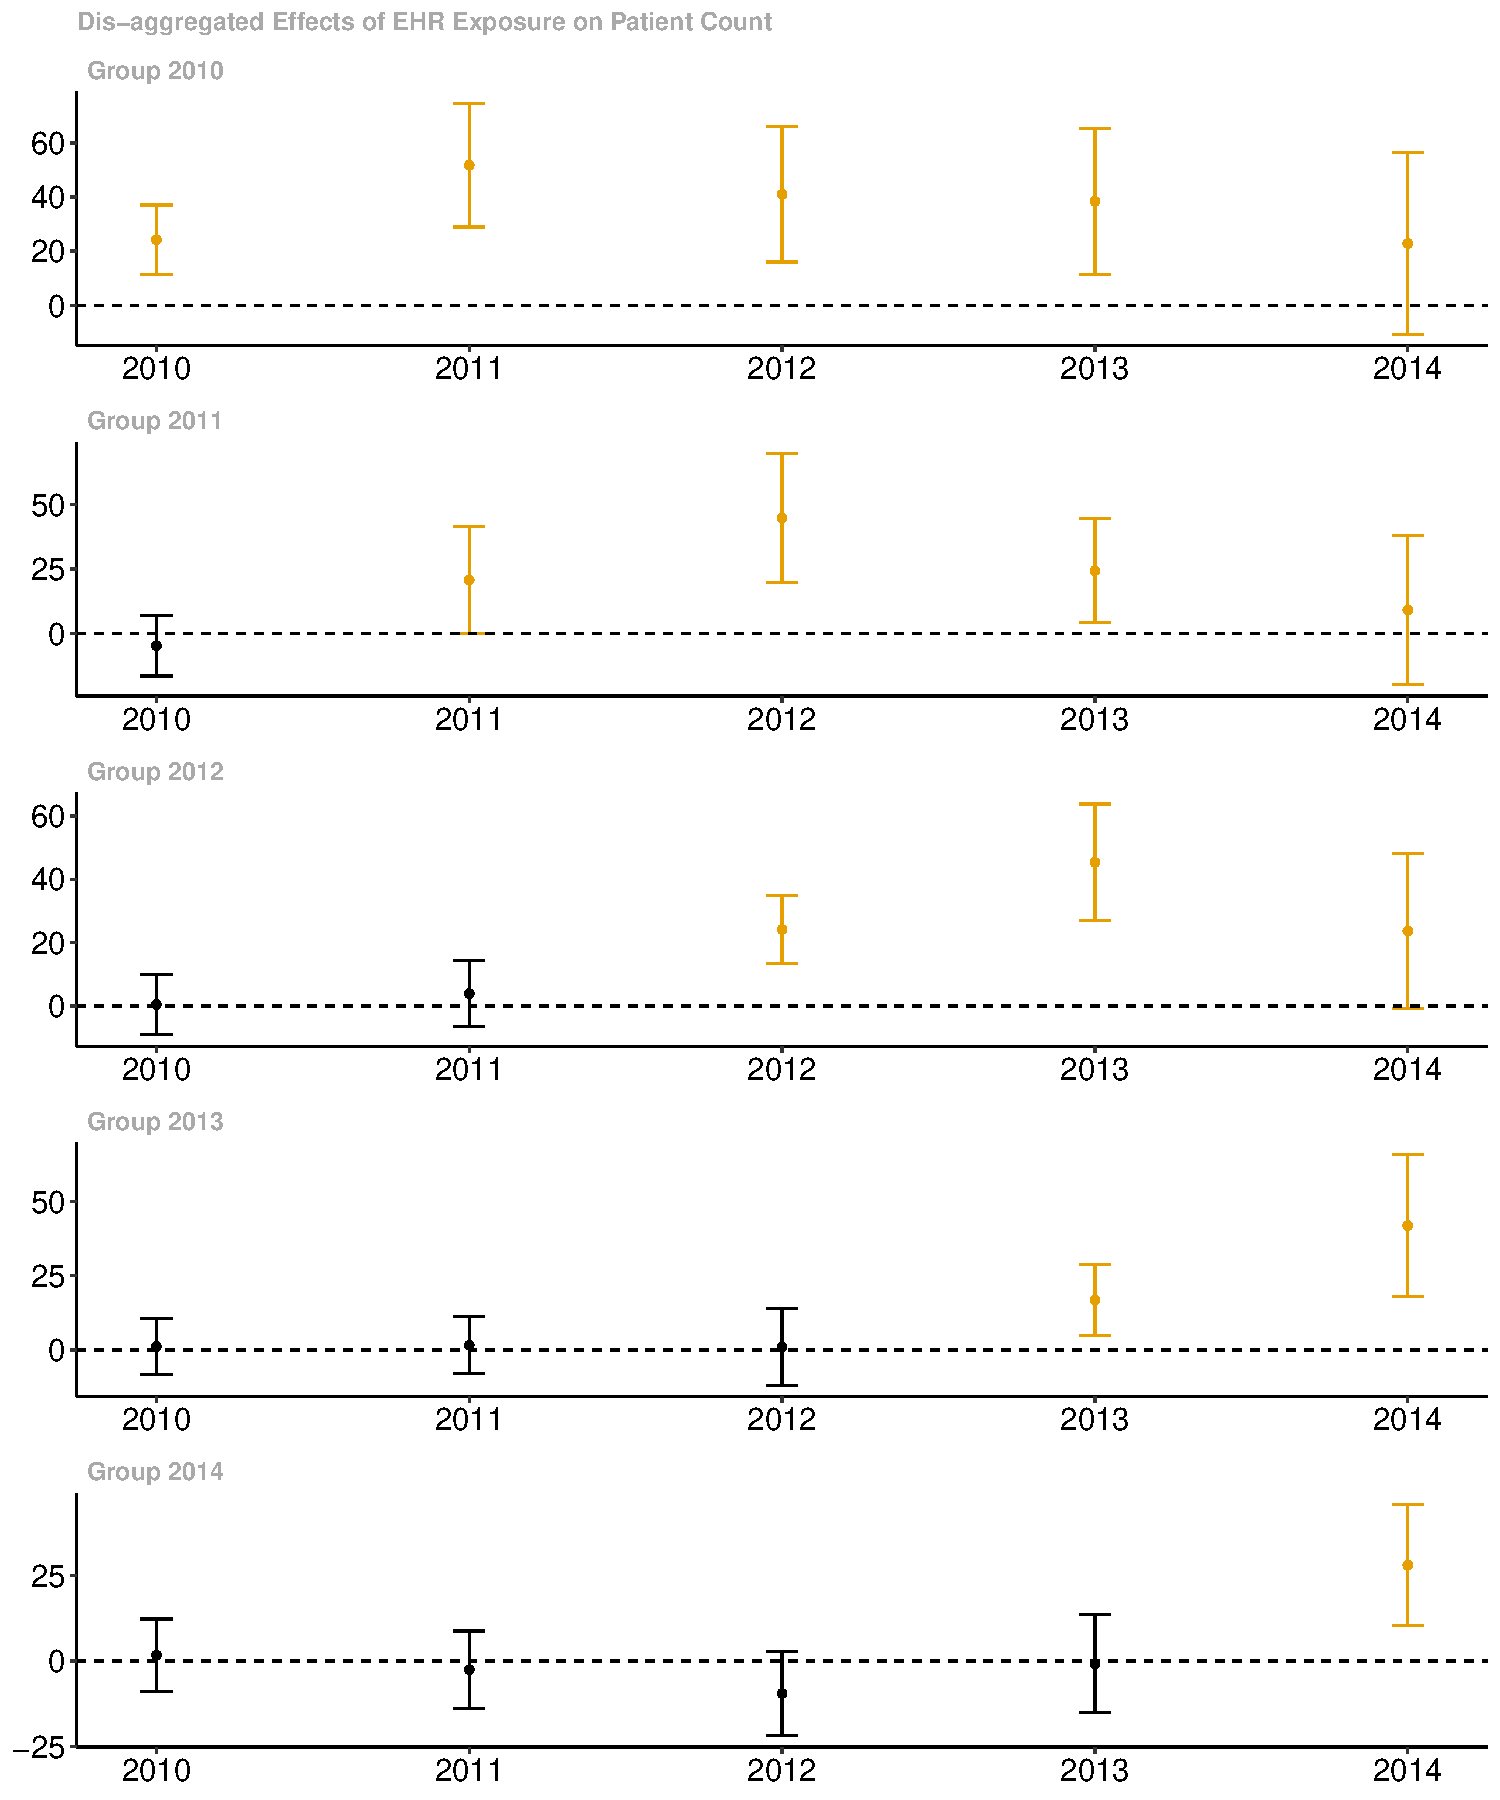
\includegraphics[scale=.25]{Objects/patient_group.pdf}
\end{frame}

\begin{frame}{Patient Count: Senior Physicians}
\begin{figure}[ht]
    \centering
    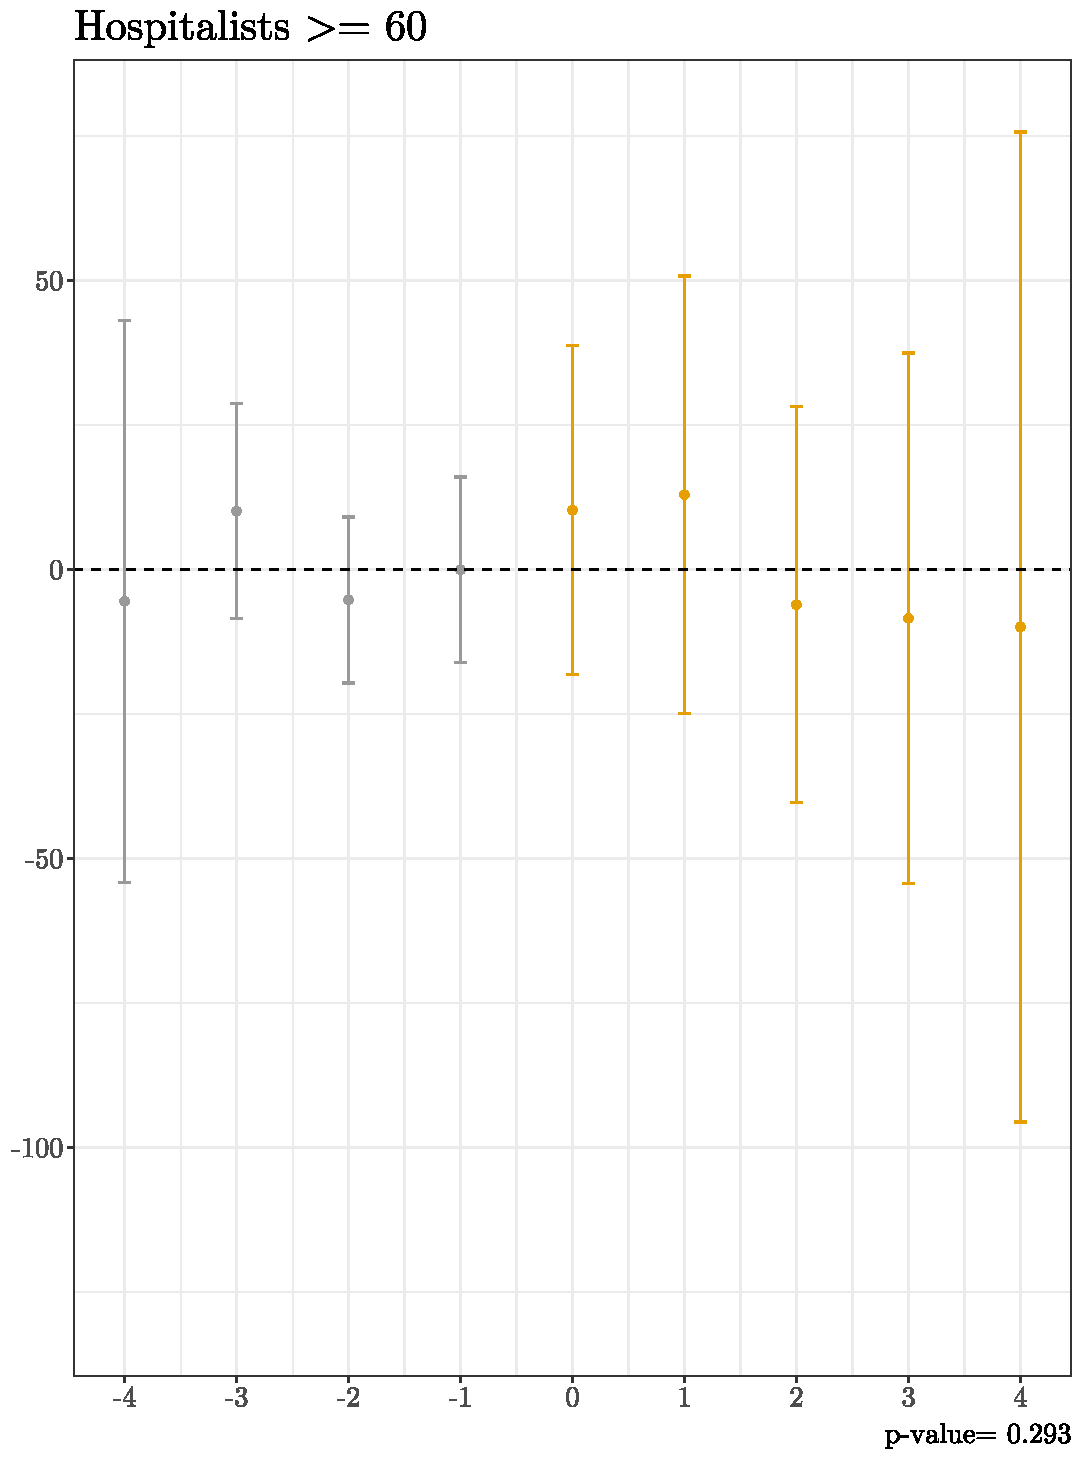
\includegraphics[scale=.4]{Objects/Presentation_patients_old.pdf}
\end{figure}
\end{frame}

\begin{frame}{Claims per Patient}
\begin{figure}[ht]
    \centering
    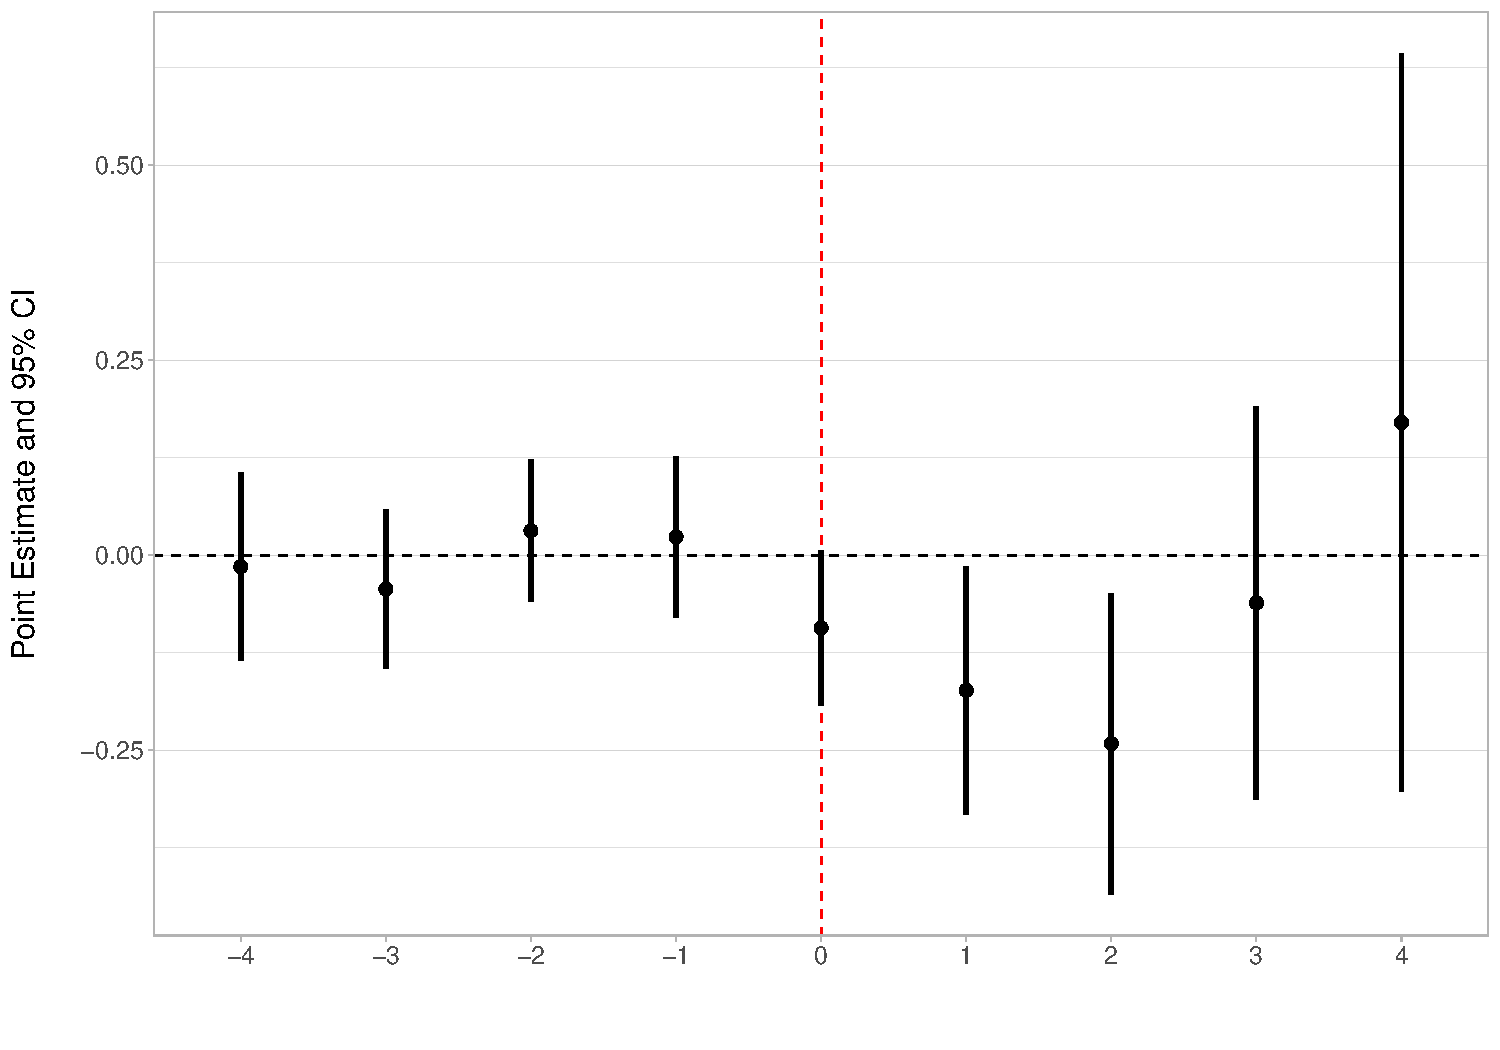
\includegraphics[scale=.35]{Objects/Presentation_claimperpatient_all.pdf}
\end{figure}
$\rightarrow$ No significant change, but a downward trend is possible
\end{frame}





\section{Conclusion}


\begin{frame}{Summary}
\begin{itemize}
    \item Evidence that physicians are changing their behavior because of this new technology, specifically through retirement or job switching
    \vspace{3mm}
    \item Little evidence of work setting changes
    \vspace{3mm}
    \item For physicians who endure through the implementation of the technology, number of patients goes up but not conclusive evidence that claims per patient goes down
    
\end{itemize}
\end{frame}

\begin{frame}{Robustness Checks}
    \begin{enumerate}
        \item Endogeneity of treatment
        \item Data assistants
        \item Limiting Years and Using Never-treated as control
        \item Anticipation
    \end{enumerate}
\end{frame}








\begin{frame}[plain]{}
\centering
    Thank you! \\
    \vspace{5mm}
    Email: hkagele@emory.edu
\end{frame}



\end{document}